\chapter{Simulations}
\label{ch:simulations}

\section{Why simulations?}

Simulations are used to check if the data we see is what we expected.



\section{Extensive air shower models}

Aires, CORSIKA or ...
Why was \corsika chosen.

It is based on various models for high/low energy hardon/electoweak
interactions; QGSJET/gheisha etc... Updated for LHC..


\subsection{Simulations catalogue}

Show in tables how many showers of each energy/primary/zenith we have.

\todo{Update plot with intermediate energies, and 'color bar'}

\begin{figure}
    \centering
    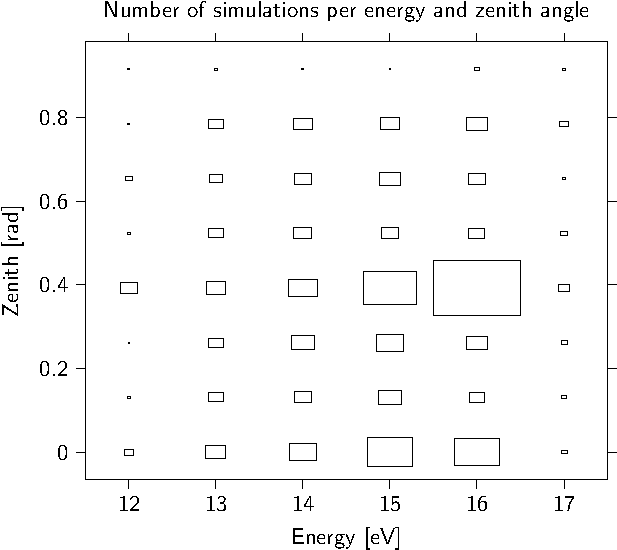
\includegraphics[width=0.7\linewidth]
        {plots/simulations/proton_energy_zenith}
    \caption{\captitle{Proton simulations overview.} The area of the
             rectangles indicate the number simulations with that energy
             and zenith combinations.}
    \label{fig:simulations_proton_energy_zenith}
\end{figure}


\section{Detector simulation}

trigger efficiency
simulations
every step eplained and understood
trigger representateren

Simulations for various starting parameters were run. The combinations
of two seeds that can be given in the input where chosen to be unique
for each simulated shower, regardless of other parameters.


\subsection{Stoomboot}

To run a significant number of simulations the local Nikhef
computer cluster 'Stoomboot' was utilized. This cluster used to have
around 300 CPUs available, but was expanded in February 2014 to 850
CPUs. Job queueing uses a fair-use policy to give each group at Nikhef
equal access to computation time.

Simulation time for each simulation is different because the number of
particles in a simulations will be different each run. Stoomboot has a
maximum job time of \SI{96}{\hour}. This allows for showers with primary
energies upto \SI{10e17}{\electronvolt}, which take around 60 hours to
complete. Lower energy showers take far less time (energy proportional
to time?), so a large sample of showers can easily be generated by
running many jobs simultaneously.

Since there are also showers of energies \SI{10e17}{\electronvolt} we
want to have some simulations at higher energies. So during the
Christmas holidays we ran 200 jobs at energies upto
\SI{10e18}{\electronvolt}. These jobs sometimes took over
\SI{400}{\hour} to complete. This was a special run where the maximum
jobs times had to be explicitly set by the administrators. In total we
used \SI{50}{\year} of compute time to generate the simulation sample.

\todo{Determine compute time used on Stoomboot}


\section{Simulations on clusters}

We have some simple simulations for flat and curved shower fronts.
Does not include particle density.
Detector/trigger/response simulations. Do we understand what we see?


\section{Realistic simulation}

\todo{Simulation with fluxes and azimuth/zenith distributions.}

\todo{Acceptance; angle, energy and particles.}

See detector response, cluster response and calibration.


\section{Analysis}

\todo{Information about shower from simulations}

Timing information, front shape, timing distribution, particle arrival times..
Air pressure dependence.

Particle density, effect of inclination..
